% Part 2 chapter carrying "Constraints on Late-Time f sigma8 Suppression from mu < 1, Sigma = 1: Planck 2018 and Large-Scale Structure"
% (Mahaffey, 19 Feb 2026) nearly in full, in its own order. Read in full 2026-10-02; re-confirmed in 50-line chunks, ledger 1-567 with no gaps. Chain numbers from mgcamb_validation/CHAIN_EXTRACTION_FINAL.csv
% (final chain files, 30 % burn-in). Checks: docs/verification/chains/LATE_TIME_GROWTH_CHECK.md.

\chapter{Late-time growth suppression: confrontation with Planck and large-scale structure}\label{ch:latetime}

\section*{Summary}
This chapter tests a scale-independent, late-time suppression of linear structure growth in the standard $\mu$--$\Sigma$ framework. The model sets
$\mu(a)<1$ for matter perturbations and keeps $\Sigma(a)=1$, so photon geodesics and the CMB acoustic structure are unchanged. The time dependence is
carried by the activation function $E(a)=\exp(1-1/a)$, which vanishes at early times and reaches unity at $a=1$, so recombination physics is preserved by
construction. With the coupling $\beta=\Omega_m/2$ the present-day coupling is $\mu(z{=}0)=0.864$, a $13.6\,\%$ reduction of the effective Newton constant
for linear growth. The model is implemented in MGCAMB and run in twelve MCMC analyses with Cobaya: Planck 2018 (TT, TE, EE and lensing) alone and with SDSS
redshift-space distortions, BAO, or Pantheon+ supernovae. With $\beta$ fixed, every combination is consistent with $\Lambda$CDM ($\Delta\chi^2$ between
$+0.56$ and $+1.73$), with the standard parameters unchanged. With the amplitude free, the posterior of $\mu_0$ reaches the upper edge of its prior ($+0.2$) in every combination; the prediction lies inside the
$90\,\%$ credible interval in all four, with $10$--$21\,\%$ of the posterior below it. $\sigma_8$ falls from $0.813$ to $0.800$ in every combination. BAO angles and supernova distances are unaffected,
as $\Sigma=1$ requires. Euclid and DESI will reach the sensitivity to detect or exclude a modification of this size.

\section{Introduction}
$\Lambda$CDM fits the CMB anisotropies and large-scale structure well, yet early- and late-time measurements of the clustering amplitude, $\sigma_8$ and
$S_8\equiv\sigma_8(\Omega_m/0.3)^{0.5}$, have stayed apart. Weak-lensing surveys report $\sigma_8$ below the Planck $\Lambda$CDM value of $\approx0.81$, a
2--3$\sigma$ difference that has persisted across experiments and pipelines (DES, KiDS, HSC). This motivates controlled late-time changes to growth that
leave the early universe alone.

The $\mu$--$\Sigma$ parameterisation (Bean and Tangmatitham 2010; Daniel et al.\ 2010; Pogosian and Silvestri 2016) encodes departures from general
relativity through $\mu(a)$, which modifies the Poisson equation for matter clustering, and $\Sigma(a)$, which modifies the lensing potential. DES, KiDS and
Euclid use it. Keeping $\Sigma=1$ preserves photon geodesics and the CMB acoustic structure while allowing growth to change.

The model examined here is
\begin{equation}
\mu(a)=\frac{H^2_{\Lambda\rm CDM}(a)}{H^2_{\Lambda\rm CDM}(a)+\beta E(a)H_0^2},\qquad E(a)=\exp\!\left(1-\frac1a\right),
\label{eq:lt_mu}\end{equation}
so that $\mu(z{=}0)=1/(1+\beta)=0.864$ for $\beta=\Omega_m/2=0.1575$ ($\Omega_m=0.315$), a $13.6\,\%$ suppression of the coupling for matter perturbations.
The form of $E(a)$ comes from integrating the decoherence rate weighted by horizon thermodynamics (Bekenstein--Hawking entropy, Gibbons--Hawking temperature,
Landauer's principle); the coupling $\beta=\Omega_m/2$ follows from the virial partition; and the rational form of Eq.~\eqref{eq:lt_mu} follows from adding the
information entropy to the Cai--Kim horizon first law (Chapters~\ref{ch:theory} and \ref{ch:virial}). None of it is fitted to data. Independently of that
derivation, the rational form is the minimal one-amplitude realisation among monotonic activation functions that vanish early and saturate at $a=1$: it keeps
$\mu\to1$ at high redshift and fixes $\mu(z{=}0)$ through $\beta$ alone. This chapter tests the phenomenology; no covariant action is assumed.

$\mu<1$ with $\Sigma=1$ has had less attention than $\mu>1$. $f(R)$ gravity, the normal branch of DGP and most scalar--tensor theories predict enhanced
growth, $\mu\ge1$ (Pogosian and Silvestri 2016). The self-accelerating branch of DGP gives $\mu<1$ with $\Sigma=1$, but it carries a ghost and is excluded
by data. A suppression moves $\sigma_8$ downward and sits in a less explored part of the $\mu$--$\Sigma$ plane.

\begin{figure}[h]\centering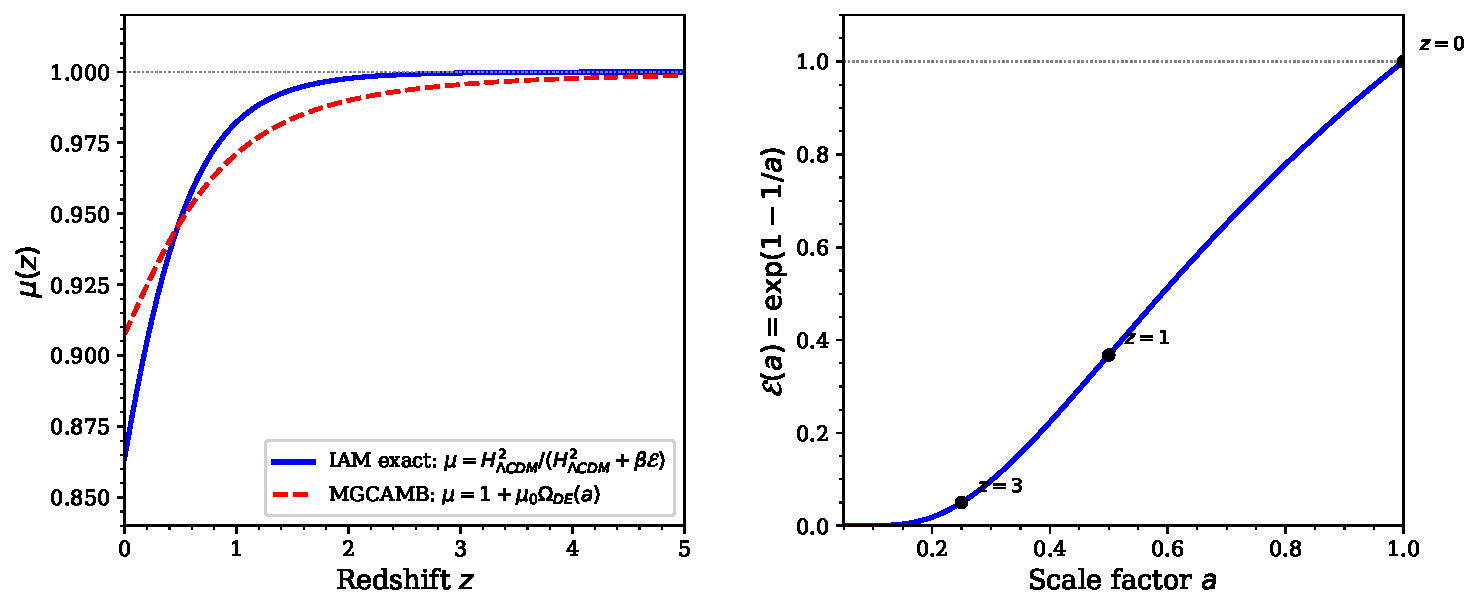
\includegraphics[width=0.85\textwidth]{figs_late_time_growth/fig_mu_profile.pdf}
\caption{Left: $\mu(z)$, exact form (Eq.~\ref{eq:lt_mu}, solid) and the MGCAMB form (Eq.~\ref{eq:lt_mgcamb}, dashed); they agree at $z=0$ and $z\gg1$ and differ by up to $2.8\,\%$ near $z\approx0.65$. Right: $E(a)=\exp(1-1/a)$, negligible above $z\approx3$ and equal to $1$ today.}\label{fig:lt_mu}\end{figure}

\section{Model and implementation}
\subsection{Modified Poisson equations}
In Fourier space,
\begin{align}
k^2\Phi&=-4\pi G\,\mu(a)\,a^2\bar\rho_m\delta_m,\\
k^2(\Phi+\Psi)&=-8\pi G\,\Sigma(a)\,a^2\bar\rho_m\delta_m,
\end{align}
with $\Phi$ and $\Psi$ the potentials in conformal Newtonian gauge, $\bar\rho_m$ the mean matter density and $\delta_m$ the density contrast. $\mu$ governs the growth
of density perturbations, $\Sigma$ the lensing potential $(\Phi+\Psi)/2$; general relativity is $\mu=\Sigma=1$. Here $\Sigma\equiv1$, so photon geodesics,
lensing and the CMB acoustic structure are standard. At fixed primordial amplitude the CMB lensing power changes by under $0.5\,\%$ (a Limber estimate gives
$0.05$--$0.3\,\%$ for $30\le L\le1000$), and the ISW contribution at $\ell<30$ stays within cosmic variance.

\subsection{MGCAMB implementation}
MGCAMB (Wang et al.\ 2023) implements the DES parameterisation
\begin{equation}
\mu(a)=1+\mu_0\,\frac{\Omega_{\rm DE}(a)}{\Omega_\Lambda},\qquad\Sigma(a)=1+\Sigma_0\,\frac{\Omega_{\rm DE}(a)}{\Omega_\Lambda},
\label{eq:lt_mgcamb}\end{equation}
with $\Omega_{\rm DE}(a)=\Omega_\Lambda/[\Omega_ma^{-3}+\Omega_\Lambda]$, so $\mu(z{=}0)=1+\mu_0$. The runs set $\mu_0=-0.13495$ and $\Sigma_0=0$.
\calc\ Eq.~\eqref{eq:lt_mgcamb} reproduces the exact form at $z=0$ ($0.865$ vs $0.864$) and at $z\gg1$; in between it suppresses slightly more, by at most
$2.8\,\%$ in $\mu$ near $z=0.65$, $2.5\,\%$ at $z=1$ and under $1\,\%$ above $z=2.5$, because $E(a)$ and $\Omega_{\rm DE}(a)$ have different transition profiles.
\emph{Notation.} $\mu_0\equiv\mu(z{=}0)-1$; $\mu_0<0$ is suppression; the prediction is $\mu_0=-0.135$.
MGCAMB settings in every run: \texttt{MG\_flag = 1}, \texttt{pure\_MG\_flag = 2}, \texttt{musigma\_par = 1}, \texttt{GRtrans = 0.001} (GR enforced below this
scale factor), $\Sigma_0=0$.

\section{Data and method}
\paragraph{Planck 2018 CMB.} Low-$\ell$ TT and EE, high-$\ell$ \texttt{plik\_lite} TTTEEE, and CMB lensing.
\paragraph{Redshift-space distortions.} The BOSS DR12 final consensus likelihood (Alam et al.\ 2017): BAO distances and $f\sigma_8$ at $z=0.38$, $0.51$
and $0.61$ with their joint covariance, which probe directly the growth that $\mu$ changes. The same runs add the eBOSS DR16 ELG, QSO and LRG likelihoods,
which are BAO distances only.
\paragraph{BAO.} SDSS DR12 and eBOSS DR16 LRG, QSO and Lyman-$\alpha$. The BAO feature is imprinted in matter, but its angular position is measured with
photons on null geodesics; with $\Sigma=1$ the angular-diameter distance and $\theta_{\rm BAO}$ are those of $\Lambda$CDM. The growth change can alter the
feature's amplitude, not its position, which is the primary observable.
\paragraph{Type Ia supernovae.} Pantheon+, 1701 light curves, $0.001<z<2.26$. In this perturbation-level model, which leaves the background unchanged,
their luminosity distances are those of $\Lambda$CDM.
\paragraph{Analysis.} Twelve chains in four data combinations (Planck: A, B, C; + RSD: D, E, F; + BAO: G, H, I; + Pantheon+: J, K, L), each with three models:
$\mu_0$ fixed at $-0.13495$ (no parameter beyond $\Lambda$CDM); $\mu_0$ free with a flat prior $[-0.5,+0.2]$; and $\Lambda$CDM ($\mu_0=\Sigma_0=0$) on the same
MGCAMB code, so any difference comes from the gravity parameter alone. The six standard parameters $\{\Omega_bh^2,\Omega_ch^2,H_0,\tau,\ln10^{10}A_s,n_s\}$ are
sampled in all runs; $\sigma_8$ and $\Omega_\Lambda$ are derived. The free-$\mu_0$ runs start at the prediction (proposal width $0.05$). Cobaya, Gelman--Rubin $R-1<0.01$; every final chain ends at $R-1\le0.0099$.

\section{Results}
$\Delta\chi^2$ is IAM fixed minus $\Lambda$CDM, from the lowest $\chi^2$ reached in each final chain; a positive value means IAM fits slightly worse. With the same
number of parameters, the likelihood ratio is $e^{-\Delta\chi^2/2}$.

\begin{table}[h]\centering\small
\caption{Planck 2018 alone (posterior means $\pm1\sigma$).}\label{tab:lt_planck}
\begin{tabular}{lccc}\hline
& $\Lambda$CDM (C) & $\mu_0$ fixed (A) & $\mu_0$ free (B)\\\hline
$H_0$ & $67.14\pm0.51$ & $67.08\pm0.53$ & $67.14\pm0.54$\\
$\sigma_8$ & $0.8143\pm0.0060$ & $0.8015\pm0.0058$ & $0.8158\pm0.0156$\\
$\mu_0$ & 0 & $-0.135$ & Table~\ref{tab:lt_free}\\
$\Delta\chi^2$ & -- & $+0.96$ & --\\\hline
\end{tabular}\end{table}
\paragraph{Planck alone.} The fixed prediction gives $\Delta\chi^2=+0.96$ (likelihood ratio $0.62$). With $\mu_0$ free the posterior (Table~\ref{tab:lt_free}) is consistent
with general relativity and with the prediction. The CMB alone is weakly sensitive to late-time growth when $\Sigma=1$.

\begin{table}[h]\centering\small
\caption{Planck + RSD.}\label{tab:lt_rsd}
\begin{tabular}{lccc}\hline
& $\Lambda$CDM (F) & $\mu_0$ fixed (D) & $\mu_0$ free (E)\\\hline
$H_0$ & $67.49\pm0.41$ & $67.49\pm0.42$ & $67.55\pm0.40$\\
$\sigma_8$ & $0.8133\pm0.0060$ & $0.8004\pm0.0060$ & $0.8166\pm0.0131$\\
$\mu_0$ & 0 & $-0.135$ & Table~\ref{tab:lt_free}\\
$\Delta\chi^2$ & -- & $+0.56$ & --\\\hline
\end{tabular}\end{table}
\paragraph{Planck + RSD.} Growth-rate data test the coupling directly. The fixed prediction gives $\Delta\chi^2=+0.56$, lower than with Planck alone: the growth data
do not penalise the suppression. $\sigma_8$ is $0.8004\pm0.0060$ against $0.8133\pm0.0060$, lower by $0.013$; the other parameters are unchanged, so the
modification acts on growth without opening degeneracies (Fig.~\ref{fig:lt_post}).
Figure~\ref{fig:lt_fs8} shows $f\sigma_8(z)$: the model is lower than $\Lambda$CDM at every redshift.
\begin{figure}[h]\centering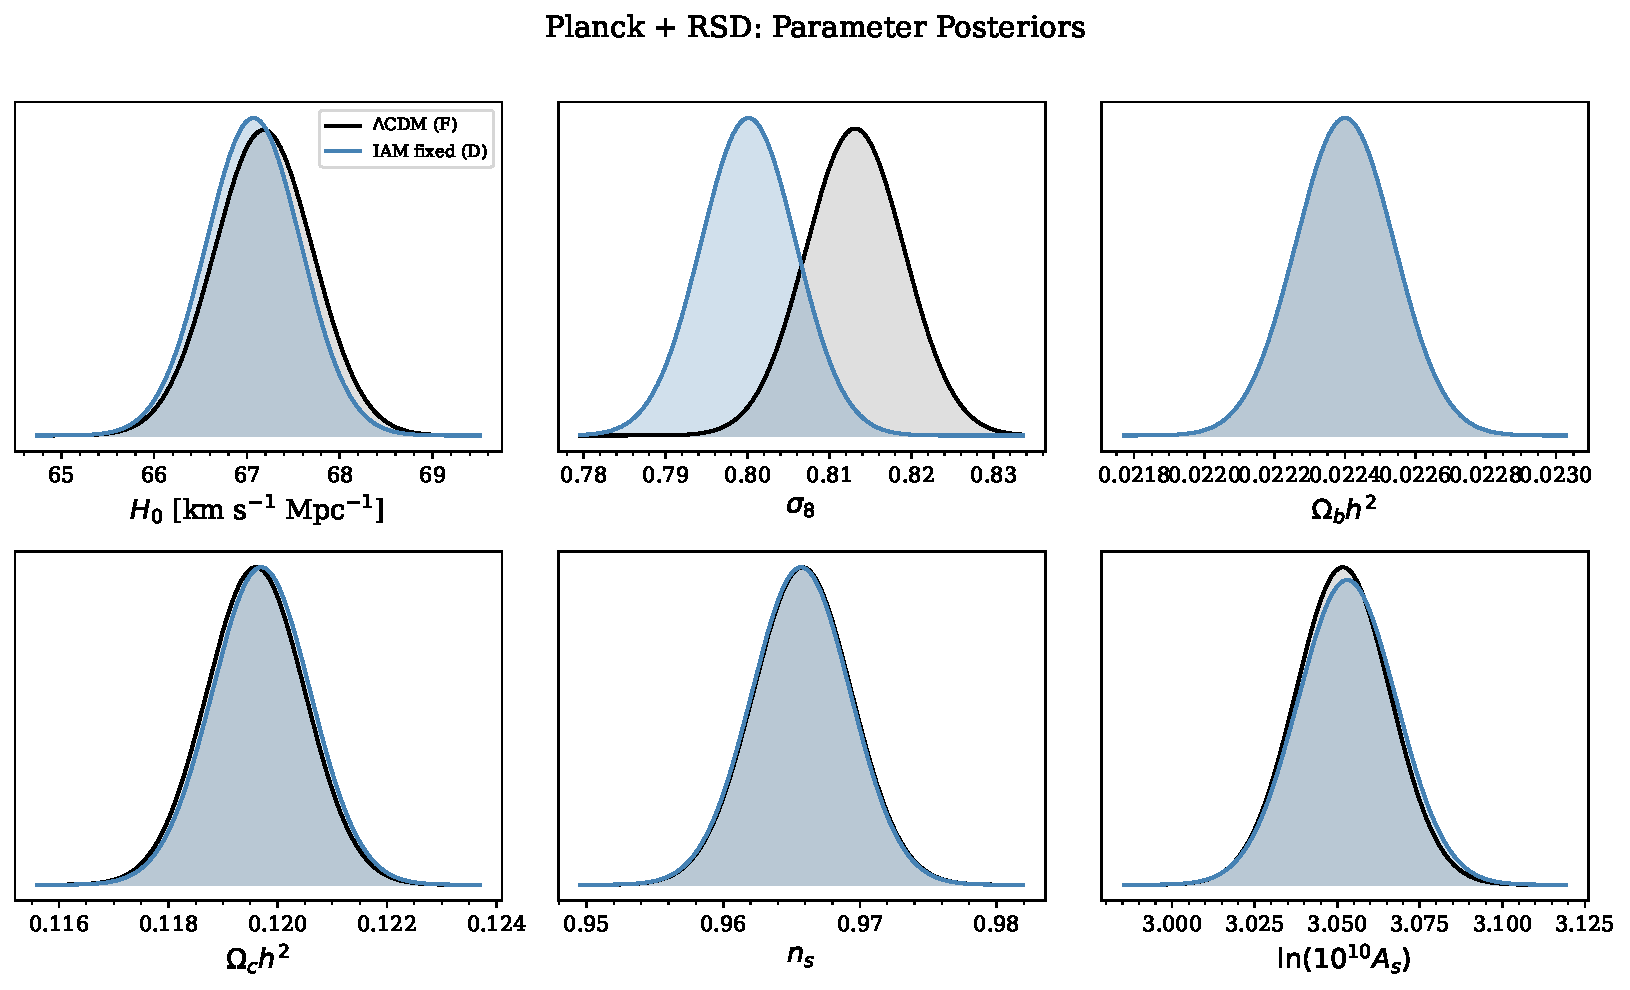
\includegraphics[width=0.85\textwidth]{figs_late_time_growth/fig_posterior_comparison.pdf}\caption{Planck + RSD posteriors, $\Lambda$CDM (grey) and $\mu_0=-0.135$ fixed (blue). Only $\sigma_8$ moves.}\label{fig:lt_post}\end{figure}
\begin{figure}[h]\centering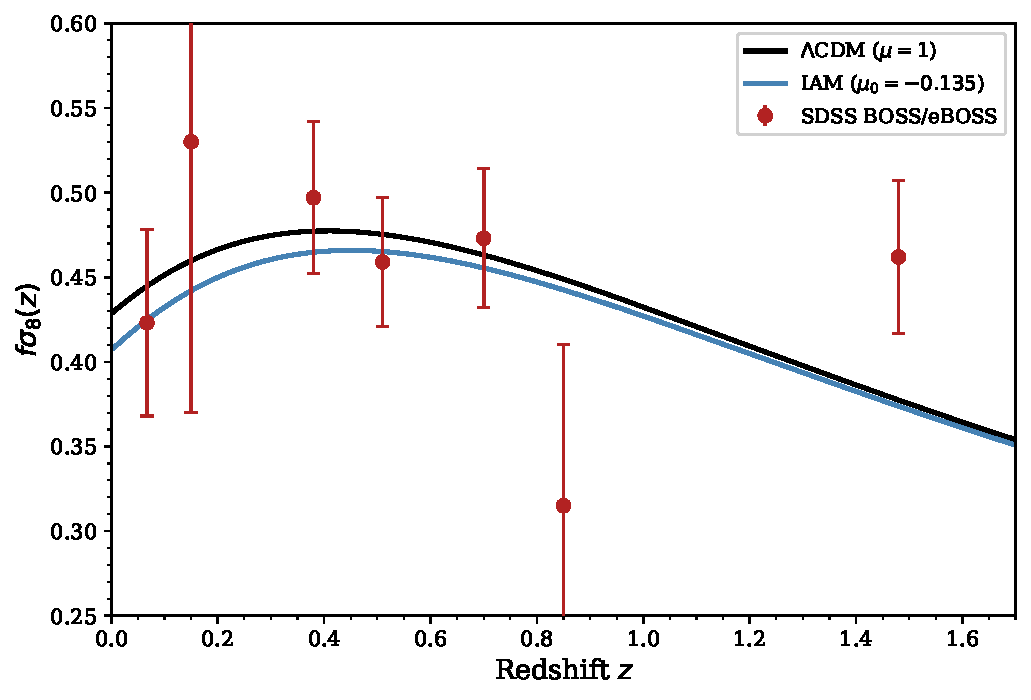
\includegraphics[width=0.7\textwidth]{figs_late_time_growth/fig_fsigma8.pdf}\caption{$f\sigma_8(z)$ for $\Lambda$CDM (black) and $\mu_0=-0.135$ (blue) with the measurements: 6dFGS ($z=0.07$), SDSS MGS ($0.15$), BOSS DR12 ($0.38$, $0.51$), eBOSS DR16 LRG ($0.70$), ELG ($0.85$) and quasars ($1.48$).}\label{fig:lt_fs8}\end{figure}

\begin{table}[h]\centering\small
\caption{Planck + BAO and Planck + Pantheon+.}\label{tab:lt_bao_sn}
\begin{tabular}{lccc|ccc}\hline
& \multicolumn{3}{c|}{Planck + BAO} & \multicolumn{3}{c}{Planck + Pantheon+}\\
& $\Lambda$CDM (I) & fixed (G) & free (H) & $\Lambda$CDM (L) & fixed (J) & free (K)\\\hline
$H_0$ & $67.56\pm0.44$ & $67.54\pm0.43$ & $67.57\pm0.45$ & $67.12\pm0.51$ & $67.00\pm0.50$ & $67.07\pm0.52$\\
$\sigma_8$ & $0.8115$ & $0.7987$ & $0.8126\pm0.0158$ & $0.8128$ & $0.7999$ & $0.8123\pm0.0164$\\
$\mu_0$ & 0 & $-0.135$ & Table~\ref{tab:lt_free} & 0 & $-0.135$ & Table~\ref{tab:lt_free}\\
$\Delta\chi^2$ & -- & $+1.73$ & -- & -- & $+1.58$ & --\\\hline
\end{tabular}\end{table}
\paragraph{Planck + BAO and Planck + Pantheon+.} BAO constrains $D_A(z)$ and $H(z)$ through the transverse and line-of-sight acoustic scales; supernovae measure
luminosity distances. With the background unchanged, both are predicted to match $\Lambda$CDM, and they do: $\Delta\chi^2=+1.73$ and $+1.58$, standard parameters
unchanged.

\begin{figure}[h]\centering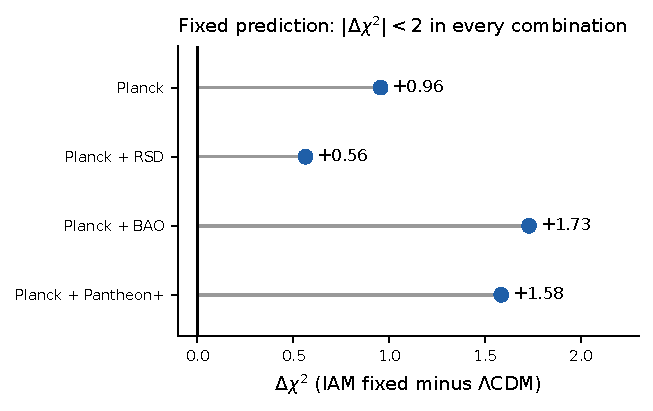
\includegraphics[width=0.6\textwidth]{figs_late_time_growth/fig_deltachi2_final.pdf}\caption{$\Delta\chi^2$ for $\mu_0=-0.135$ fixed, relative to $\Lambda$CDM, in each data combination (final chain files).}\label{fig:lt_dchi2}\end{figure}
\begin{table}[h]\centering\small
\caption{Summary, $\mu_0$ fixed at the prediction.}\label{tab:lt_summary}
\begin{tabular}{lcccc}\hline
Data & $\Delta\chi^2$ & $\sigma_8$ ($\Lambda$CDM) & $\sigma_8$ (IAM) & $\Delta\sigma_8/\sigma_8$\\\hline
Planck & $+0.96$ & $0.8143$ & $0.8015$ & $-1.6\,\%$\\
Planck + RSD & $+0.56$ & $0.8133$ & $0.8004$ & $-1.6\,\%$\\
Planck + BAO & $+1.73$ & $0.8115$ & $0.7987$ & $-1.6\,\%$\\
Planck + Pantheon+ & $+1.58$ & $0.8128$ & $0.7999$ & $-1.6\,\%$\\\hline
\end{tabular}\end{table}

\subsection{The free amplitude}
\begin{table}[h]\centering\small
\caption{$\mu_0$ free, flat prior $[-0.5,+0.2]$: posterior median, lower end of the $90\,\%$ credible interval (the upper end is the prior edge), and the
posterior probability below the prediction.}\label{tab:lt_free}
\begin{tabular}{lccc}\hline
Data & median & $90\,\%$ lower bound & $P(\mu_0<-0.135)$\\\hline
Planck & $+0.059$ & $-0.305$ & $0.17$\\
Planck + RSD & $+0.064$ & $-0.204$ & $0.10$\\
Planck + BAO & $+0.047$ & $-0.304$ & $0.18$\\
Planck + Pantheon+ & $+0.030$ & $-0.342$ & $0.21$\\\hline
\end{tabular}\end{table}
\calc\ In every combination the posterior rises to the prior's upper edge: $17$--$21\,\%$ of it lies above $+0.15$ (Fig.~\ref{fig:lt_mu0}). A mean and standard
deviation therefore describe the prior range as much as the data, and the table gives the median and one-sided bound instead. The prediction lies inside
every $90\,\%$ interval, as does general relativity. The direction of the pull is upward, toward enhanced growth; a run with a wider prior would show where the
posterior turns over.
\begin{figure}[h]\centering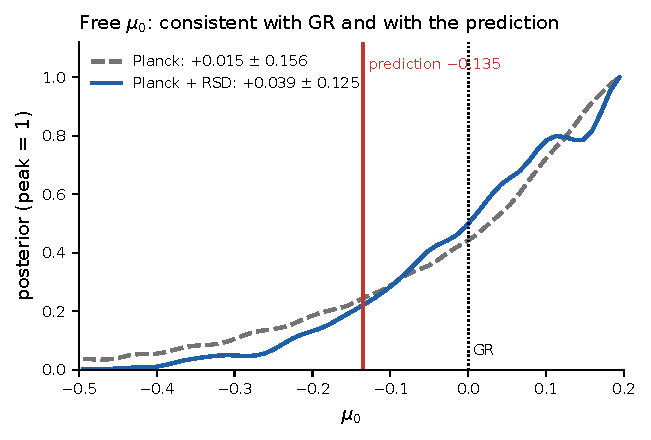
\includegraphics[width=0.65\textwidth]{figs_late_time_growth/fig_mu0_posterior_final.pdf}\caption{Posterior of $\mu_0$ with the amplitude free, Planck (dashed) and Planck + RSD (solid), from the final chain files. The prior ends at $+0.2$; the vertical line marks the prediction.}\label{fig:lt_mu0}\end{figure}

\section{Discussion}
\subsection{Compatibility with current data}
The main result is that a zero-parameter prediction, a $13.6\,\%$ weakening of the coupling for matter perturbations at $z=0$ from $\beta=\Omega_m/2$,
passes the full Planck 2018 likelihood with no tension, and stays that way when growth-rate data, which probe the modification directly, are added. Most proposed
late-time changes to gravity are excluded or tightly limited by Planck, so this consistency was not guaranteed.

\subsection{The $\sigma_8$ shift}
$\sigma_8$ falls from $\approx0.813$ to $\approx0.800$ ($1.6\,\%$) in every combination. It follows from $\mu<1$: the weaker source term in the Poisson equation slows
growth and lowers $\sigma_8$, while the primary CMB spectrum is unchanged because $\Sigma=1$. The size is set by $\mu_0=-0.135$ alone; no late-time clustering datum
was used, and the direction, toward the weak-lensing values, was not an input. KiDS-1000 reports $S_8=0.759^{+0.024}_{-0.021}$ and DES Y3 $S_8=0.776\pm0.017$.
Whether this shift reduces the CMB--lensing difference quantitatively needs a joint analysis with the KiDS and DES likelihoods.

\subsection{Comparison with other modified-gravity results}
\observed\ Current constraints in the same parameterisation: DES Y3 with external data, $\mu_0=0.08^{+0.21}_{-0.19}$ (DES Y3 alone does not constrain $\mu_0$;
Abbott et al.\ 2023); DESI 2024 full shape with BAO and BBN, $\mu_0=0.11^{+0.45}_{-0.54}$, and with CMB and DES Y3, $0.04\pm0.22$ (DESI Collaboration 2025);
ACT + WMAP + SDSS + SN, $\mu_0=0.02\pm0.19$ (Andrade et al.\ 2024). The prediction $\mu_0=-0.135$ is inside every one.

\subsection{What next-generation surveys can do}
\begin{table}[h]\centering\small
\caption{Projected sensitivity to $\mu_0=-0.135$ with $\Sigma=1$ imposed (Fisher estimates from published survey specifications).}\label{tab:lt_forecast}
\begin{tabular}{lcc}\hline
Survey & $\sigma(\mu_0)$ & $|\mu_0|/\sigma$\\\hline
Planck + RSD (this chapter) & $\sim0.12$ & $\sim1.1$\\
Euclid, pessimistic & $\sim0.06$ & $\sim2.2$\\
Euclid, optimistic & $\sim0.04$ & $\sim3.4$\\
DESI Year 5, $f\sigma_8$ only & $\sim0.10$ & $\sim1.4$\\
Euclid + DESI Y5 & $\sim0.025$ & $\sim5.4$\\\hline
\end{tabular}\end{table}
\prediction\ Euclid alone tests the amplitude at about $3\sigma$; with DESI Year 5 the combined constraint reaches $\sigma(\mu_0)\approx0.025$. Letting $\Sigma_0$ float as
well would weaken these numbers.

\subsection{Limits of this analysis}
\begin{enumerate}
\item \emph{Phenomenological.} Only the $\mu$--$\Sigma$ form is tested here; the derivation of $E(a)$ and $\beta$ is in Chapters~\ref{ch:theory} and \ref{ch:virial}.
The results stand on their own: any model with $\mu_0\approx-0.135$ and $\Sigma=1$ faces the same tests.
\item \emph{Perturbations only.} The background is $\Lambda$CDM throughout.
\item \emph{MGCAMB form.} Eq.~\eqref{eq:lt_mgcamb} matches the exact $\mu$ at $z=0$ and high $z$ and departs from it by up to $2.8\,\%$ near $z\approx0.65$; small now,
relevant at Euclid precision.
\item \emph{Linear scales.} Cluster counts and small-scale lensing need N-body simulations or validated fitting functions.
\item \emph{Weak-lensing likelihoods.} Not yet included; a joint analysis is the next step.
\end{enumerate}

\section{Conclusions}
\begin{enumerate}
\item A fixed $13.6\,\%$ suppression of the coupling at $z=0$ is consistent with Planck 2018 ($\Delta\chi^2=+0.96$) and with Planck + SDSS growth data ($+0.56$).
\item $\sigma_8$ moves from $\approx0.813$ to $\approx0.800$ with no other parameter degraded.
\item With $\mu_0$ free, the prediction lies inside the $90\,\%$ credible interval in every combination; the posterior leans toward positive $\mu_0$ and reaches the prior edge.
\item BAO and supernova distances are unaffected, as a perturbation-level change with $\Sigma=1$ requires.
\item Euclid and DESI will reach the sensitivity to detect or exclude a change of this size.
\end{enumerate}
$\mu<1$ with $\Sigma=1$ lies in a less explored region than $f(R)$, DGP and most scalar--tensor theories; current data do not disfavour it, and it makes specific
predictions for the next surveys. All chains, Cobaya configuration files and scripts are in the repository (\texttt{mgcamb\_validation/}).
